\documentclass[border=10pt]{standalone} %\documentclass[tikz]{standalone}
\usepackage{pgfplots}
\usepackage{tikz}
\usetikzlibrary{calc,decorations.pathmorphing,shapes}
\usepackage{amsmath}
\usepackage{bm}
\usepackage{graphicx}
\usepackage{graphics}
\usepackage{xcolor}
%\pgfplotsset{compat=1.10}
\usepackage{pgfplots}
%\usepackage{ifthenelse}


\begin{document}

%\begin{figure}
%\centering\makebox[\textwidth]{
\begin{tikzpicture}[scale=2,cap=round]
% Local definitions
  \def\fiberrad{0.5cm}	% Radius of the nanofiber.
  \def\comprad{0.15cm}	% Compressed radius of the nanofiber in the view angle.
  \def\fiberleftx{-4cm}	% The x-coordiante of the center of the left surface of the fiber.
  \def\fiberlefty{0cm}	% The y-coordiante of the center of the left surface of the fiber.
  \def\fiberlength{8cm} % The length of the fiber.
  \def\atomdist{0.5cm}	% drp at r'
  
  \coordinate (O) at (0,0);		% origin
  \coordinate (LO) at (\fiberleftx,\fiberlefty); % Center of the left-side surface of the nanofiber.
  \coordinate (RO) at (\fiberleftx+\fiberlength,\fiberlefty); % Center of the right-side surface of the fiber.
  \coordinate (A) at ({\fiberleftx},{\fiberlefty+\fiberrad});	% Top-left point of the nanofiber.
  \coordinate (B) at ({\fiberleftx+\fiberlength},{\fiberlefty+\fiberrad});	% Top-right point of the nanofiber.
  \coordinate (C) at ({\fiberleftx+\fiberlength},{\fiberlefty-\fiberrad});	% Bottom-right point of the fiber.
  \coordinate (D) at ({\fiberleftx},{\fiberlefty-\fiberrad});	% Bottom-left point of the nanofiber.

  % Colors
%  \colorlet{atomorange}{RGB}{238,97,26}
  \definecolor{myorange}{RGB}{238,97,26}

  % Styles
%  \tikzstyle{axes}=[]
%  \tikzstyle{important line}=[very thick]
%  \tikzstyle{information text}=[rounded corners,fill=red!10,inner sep=1ex]

  % The graphic
  % help grid
%  \draw[style=help lines,step=0.5cm] (-2.0,-2.0) grid (2.0,2.0);
  
  % Import field intensity plot.
   \begin{scope} %[xshift=-4cm]  
         \draw (-4cm, 0cm)  node  {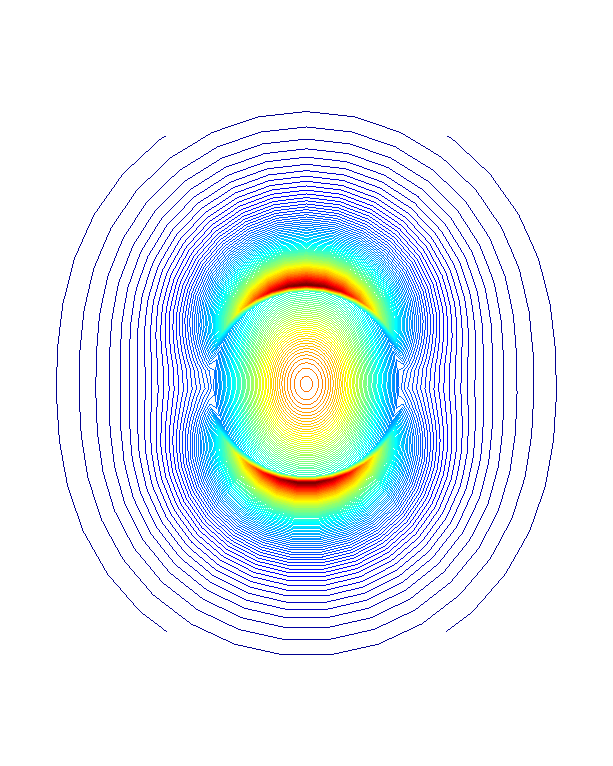
\includegraphics[width=2.3cm,height=8.5cm]{IntensityContour}};
   \end{scope}
         
    \draw [->, decorate, decoration={snake,pre length =4pt, post length=4pt}] (-3.5cm, 0.65cm) --  
    (-2.5cm,0.65cm)   node [midway, sloped, above]  {Guided} ;
    \draw [->, decorate, decoration={snake,pre length =4pt, post length=4pt}] (-3.5cm, -0.65cm) --  
         (-2.5cm,-0.65cm)   node [midway, sloped, below]  {Guided} ;
         
  \begin{scope} % Draw the fiber.
  	% Left-side surface.
   % \fill[left color=purple!50!black,right color=purple!10,middle 
%color=purple,shading=axis,opacity=0.25] (LO) circle ({\comprad} and {\fiberrad});
    % Outer edge.
    \fill[left color=purple!50!black,right color=purple!50!black,middle 
color=purple!50,shading=axis,opacity=0.25] (A) -- (B) arc (90:270:{\comprad} and {\fiberrad}) -- (D) arc 
(270:90:{\comprad} and {\fiberrad});
    % Right-side surface.
    \fill[top color=purple!90!,bottom color=purple!2,middle color=purple!30,shading=axis,opacity=0.25] 
(RO) circle [x radius={\comprad}, y radius = {\fiberrad}];
    % Draw lines of all edges.
    \draw (A) -- (B);
    \draw  (RO) circle [x radius = {\comprad}, y radius =  {\fiberrad}];
    \draw (C) -- (D) arc (270:90:{\comprad} and {\fiberrad}); 
    \draw[dashed] (A) arc (90:-90:{\comprad} and {\fiberrad});
  \end{scope}
  
  % Draw atoms and radiation lines.
  \pgfmathsetmacro{\opacVal}{0.8}
  \foreach \i in {1,2,...,6}{
    \pgfmathsetmacro{\x}{((\i-1) * 1.0 -2.0)}
      \foreach \j in {-1,1}{
        \pgfmathsetmacro{\y}{\j *1.1  }
        %    Draw atom balls.
        \shade [ball color = myorange, opacity = \opacVal] (\x cm, \y cm) circle (0.1cm);
        \node (rightabovestart) at  (\x+0.05,\y+\j*0.05) {};
        \node (rightaboveend) at (\x+0.9,\y+\j*0.9) {};
        \node (bottomstart) at (\x,\y-\j*0.1) {};
        \node (bottomend) at (\x+0.9,\y-\j*0.1-\j*0.3) {};
        \node (leftmid) at (\x-0.05,\y) {};
        \draw [->, decorate, decoration=snake] (rightabovestart) -- (rightaboveend) node [midway, sloped, 
        above] {Radiative} ;
        \pgfmathifthenelse{\j==1}{"\noexpand\draw [->, decorate, decoration={snake,pre length =4pt,post 
        length=4pt}]  (bottomstart) ..  controls +(up:-\j*0.55cm)  and +(left:0.15cm) ..  (bottomend)   node 
        [midway, sloped,above]  {Guided} ;"}
                {"\noexpand\draw [->,  decorate, decoration={snake,pre length =4pt,post length=4pt}] 
                (bottomstart) .. controls +(up:-\j*0.55cm) 
                        and +(left:0.15cm) ..  (bottomend)   node [midway, sloped,below]  {Guided} ;"}
          \pgfmathresult;
%        \draw [-<, decorate, decoration={snake,pre length =4pt}] (bottomstart) .. controls +(up:-\j*0.5cm) 
%        and +(left:0.2cm) ..  (bottomend)   node [midway, sloped,above]  {Guided} ;
        \draw [<->] (leftmid) to [out=140, in=230, looseness=12] (leftmid) node [sloped,left] 
        {$\boldsymbol{\alpha}$};
    }}
    
    % Draw some dots at the right-side end.
    \draw (4cm,1.1cm) node {$\boldsymbol{\cdots}$};
    \draw (4cm,-1.1cm) node {$\boldsymbol{\cdots}$};
    \draw (4.5cm,0.5cm) node {$\boldsymbol{\cdots}$};
    \draw (4.5cm,-0.5cm) node {$\boldsymbol{\cdots}$};
    
\end{tikzpicture} 
%}
%\caption{Diagram for the nanofiber project.}
%\label{fig:nanofibertrappedatoms}
%\end{figure}

\end{document}